\documentclass[12pt,a4paper,oneside]{book}

\usepackage[utf8]{inputenc}
\usepackage[T1]{fontenc}
\usepackage{lmodern}
\usepackage{graphicx}
\usepackage{amsmath,amssymb}
\usepackage{geometry}
\usepackage{hyperref}
\usepackage{xcolor}
\usepackage{listings}
\usepackage{microtype}
% --- additions for diagrams, tables and captions ---
\usepackage{tikz}
\usetikzlibrary{shapes.geometric,shapes.multipart,arrows.meta,positioning,fit,calc}
\usepackage{float}
\usepackage{caption}
\usepackage{booktabs}
\usepackage{array}

\geometry{margin=1in}
\setlength{\emergencystretch}{3em}

\makeatletter
\newcommand{\chapterauthor}[1]{%
  {\parindent0pt\vspace*{-15pt}%
  \linespread{1.1}\large\itshape\begin{flushright}#1\end{flushright}%
  \par\nobreak\vspace*{25pt}}
  \@afterheading%
}
\makeatother

% --- code listing style ---
\definecolor{codebg}{RGB}{248,248,248}
\definecolor{codekw}{RGB}{0,0,160}
\definecolor{codecm}{RGB}{0,120,0}
\definecolor{codestr}{RGB}{160,30,30}
\lstdefinestyle{cpp}{
  language=C++,
  basicstyle=\ttfamily\footnotesize,
  keywordstyle=\color{codekw}\bfseries,
  commentstyle=\color{codecm}\itshape,
  stringstyle=\color{codestr},
  backgroundcolor=\color{codebg},
  frame=single, rulecolor=\color{black!30},
  numbers=left, numberstyle=\tiny\color{black!50}, numbersep=6pt,
  breaklines=true, breakatwhitespace=true,
  showstringspaces=false, tabsize=4,
  captionpos=b, xleftmargin=1.5em, framexleftmargin=1.5em
}
\lstset{style=cpp}

% --- UML helpers (pure TikZ) ---
\tikzset{
  umlclass/.style={rectangle split, rectangle split parts=3, draw, fill=white,
    font=\scriptsize, text width=5.2cm, align=left, inner sep=3pt},
  usecase/.style={ellipse, draw, fill=white, font=\footnotesize, minimum width=3.4cm,
    minimum height=0.8cm, align=center},
  act/.style={rectangle, rounded corners=6pt, draw, fill=white, font=\footnotesize,
    minimum width=4.2cm, minimum height=0.7cm, align=center},
  dec/.style={diamond, draw, fill=white, aspect=2.2, font=\scriptsize, inner sep=1pt, align=center},
  flow/.style={-{Stealth[length=2.2mm]}, thick},
  assoc/.style={-, thick},
  compo/.style={{Diamond[fill=black,length=3mm,width=2mm]}-, thick},
  aggr/.style={{Diamond[open,length=3mm,width=2mm]}-, thick},
  depend/.style={-{Stealth[length=2mm]}, dashed, thick},
  msg/.style={-{Stealth[length=2mm]}, thick},
  ret/.style={-{Stealth[length=2mm]}, dashed},
}
\newcommand{\actor}[2]{% #1 node name, #2 label
  \begin{scope}[shift={(#1)}]
    \draw[thick] (0,0.55) circle (0.18);
    \draw[thick] (0,0.37) -- (0,-0.1);
    \draw[thick] (-0.3,0.2) -- (0.3,0.2);
    \draw[thick] (0,-0.1) -- (-0.22,-0.5);
    \draw[thick] (0,-0.1) -- (0.22,-0.5);
    \node[font=\footnotesize, below] at (0,-0.5) {#2};
  \end{scope}}

\begin{document}

\mainmatter

% =====================================================================
% C++ OOP Mini-Project Chapter
% File: ProjectNumber_ShortName.tex
% =====================================================================

\chapter{Inventory Management System}
\chapterauthor{Himanshu Gunwant (251127) \\ Raj Aryan Mahato (251145)}

\section{Introduction and Problem Statement}
Small shops, college stores and laboratories often track their stock in notebooks or
spreadsheets. This leads to incorrect quantities, no record of who moved stock and when,
duplicate product entries, and no warning when an item is about to run out. Anyone who can
open the spreadsheet can also change any value, so there is no access control.

The \textbf{Inventory Management System} solves this with a single, centralised C++17
backend that exposes a REST API over HTTP and stores data in an SQLite database. A
lightweight browser frontend (``Stockroom'') is served by the same backend, so the complete
workflow runs end to end: the browser sends JSON requests, the C++ server validates them,
applies the business rules inside a database transaction, and returns JSON responses.

From an end-user perspective the system lets a signed-in user:
\begin{itemize}
    \item see a dashboard with the number of items, the total stock value and the number of low-stock items;
    \item browse and search items by name, SKU or category, with pagination;
    \item record \emph{stock in} (goods received) and \emph{stock out} (goods issued) with an optional note;
    \item view the full history of stock movements; and
    \item (administrators only) manage categories, suppliers, items and user accounts.
\end{itemize}

\paragraph{Software requirements.} C++17 compiler, CMake 3.20+, the Crow HTTP framework,
nlohmann/json and SQLite~3 (the last three are fetched automatically by CMake), and any
modern web browser.

\section{Scope and Feature Set}
\begin{itemize}
    \item \textbf{Authentication:} users register and log in with email and password.
      Passwords are stored as salted SHA-256 hashes, and the server issues an
      HMAC-SHA-256 signed bearer token that expires after 24 hours.
    \item \textbf{Role-based authorisation:} two roles, \texttt{admin} and \texttt{staff}.
      Admins manage master data and users; staff can view items and record stock movements.
    \item \textbf{Category and supplier management:} full CRUD on categories and suppliers.
    \item \textbf{Item management:} CRUD on items with a unique SKU, unit price, current quantity
      and reorder level. Supports search, category filters and pagination.
    \item \textbf{Transactional stock movements:} \texttt{POST /api/stock/in} and
      \texttt{/api/stock/out} update the quantity and write a movement record atomically.
      A stock-out larger than the available quantity is rejected (HTTP 409).
    \item \textbf{Movement history:} every change is logged with item, type, quantity, note, user and timestamp.
    \item \textbf{Low-stock monitoring:} lists the items whose quantity is at or below their reorder level.
    \item \textbf{Dashboard:} total items, total stock value, low-stock count and the five latest movements.
    \item \textbf{Web frontend:} a dependency-free HTML/CSS/JavaScript single-page interface,
      served by the backend at \texttt{http://localhost:8080}.
\end{itemize}

\begin{table}[H]
\centering
\caption{REST API endpoints}
\label{tab:api}
\small
\begin{tabular}{@{}>{\ttfamily}l >{\ttfamily}l l@{}}
\toprule
\textrm{\textbf{Method}} & \textrm{\textbf{Endpoint}} & \textbf{Access} \\
\midrule
GET  & /api/health                 & Public \\
POST & /api/auth/register          & First user / Admin \\
POST & /api/auth/login             & Public \\
GET  & /api/auth/me                & Authenticated \\
GET, POST & /api/categories        & Auth / Admin \\
PUT, DELETE & /api/categories/\{id\} & Admin \\
GET, POST & /api/suppliers         & Auth / Admin \\
PUT, DELETE & /api/suppliers/\{id\}  & Admin \\
GET, POST & /api/items             & Auth / Admin \\
GET, PUT, DELETE & /api/items/\{id\} & Auth / Admin \\
GET  & /api/items/low-stock        & Authenticated \\
POST & /api/stock/in, /api/stock/out & Authenticated \\
GET  & /api/stock/movements        & Authenticated \\
GET  & /api/dashboard              & Authenticated \\
\bottomrule
\end{tabular}
\end{table}

\section{System Architecture}
The backend follows a layered architecture (Figure~\ref{fig:arch}). HTTP handling, business
logic and database access are kept in separate modules, so each layer depends only on the
one below it.

\begin{figure}[H]
\centering
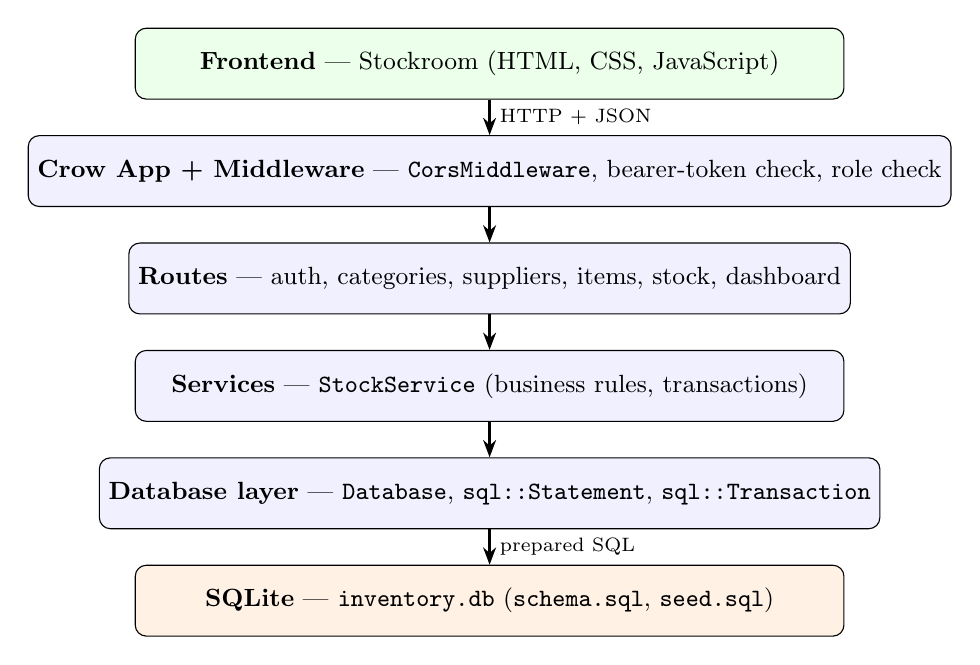
\begin{tikzpicture}[
  layer/.style={draw, rounded corners, fill=blue!6, minimum width=9cm, minimum height=0.9cm,
    font=\small, align=center},
  node distance=0.45cm]
  \node[layer, fill=green!8] (fe) {\textbf{Frontend} --- Stockroom (HTML, CSS, JavaScript)};
  \node[layer, below=of fe] (mw) {\textbf{Crow App + Middleware} --- \texttt{CorsMiddleware}, bearer-token check, role check};
  \node[layer, below=of mw] (rt) {\textbf{Routes} --- auth, categories, suppliers, items, stock, dashboard};
  \node[layer, below=of rt] (sv) {\textbf{Services} --- \texttt{StockService} (business rules, transactions)};
  \node[layer, below=of sv] (db) {\textbf{Database layer} --- \texttt{Database}, \texttt{sql::Statement}, \texttt{sql::Transaction}};
  \node[layer, below=of db, fill=orange!10] (sq) {\textbf{SQLite} --- \texttt{inventory.db} (\texttt{schema.sql}, \texttt{seed.sql})};
  \draw[flow] (fe) -- node[right, font=\scriptsize]{HTTP + JSON} (mw);
  \draw[flow] (mw) -- (rt);
  \draw[flow] (rt) -- (sv);
  \draw[flow] (sv) -- (db);
  \draw[flow] (db) -- node[right, font=\scriptsize]{prepared SQL} (sq);
\end{tikzpicture}
\caption{Layered architecture of the Inventory Management System}
\label{fig:arch}
\end{figure}

\paragraph{Database design.} The relational schema has five tables: \texttt{users},
\texttt{categories}, \texttt{suppliers}, \texttt{items} and \texttt{stock\_movements}.
\texttt{items} references \texttt{categories} and \texttt{suppliers}
(\texttt{ON DELETE SET NULL}), and \texttt{stock\_movements} references \texttt{items}
(\texttt{ON DELETE CASCADE}) and \texttt{users}. \texttt{CHECK} constraints enforce
non-negative prices and quantities, positive movement quantities, and valid roles and movement types.

\section{Object-Oriented Architecture}
The project uses C++ classes to model resources, hide implementation details and manage
resources safely. The OOP principles applied are:

\begin{itemize}
  \item \textbf{Encapsulation:} \texttt{TokenStore} keeps its token map, HMAC secret and mutex
    \texttt{private}, and exposes only \texttt{issue()} and \texttt{find()}. \texttt{Database}
    hides the raw \texttt{sqlite3*} handle behind a \texttt{std::unique\_ptr}.
  \item \textbf{Abstraction:} route handlers call \texttt{StockService::move()} without knowing
    the SQL or locking logic behind it. The \texttt{sql} helpers (\texttt{prepare}, \texttt{bindText},
    \texttt{bindInt}) hide the low-level SQLite C API.
  \item \textbf{RAII (constructors and destructors):} \texttt{Database} opens the connection in its
    constructor and a custom deleter closes it. \texttt{sql::Transaction} begins a transaction
    in its constructor and automatically rolls back in its destructor unless \texttt{commit()}
    was called. Every \texttt{sqlite3\_stmt} is wrapped in a \texttt{unique\_ptr} with
    \texttt{StatementDeleter}.
  \item \textbf{Polymorphism:} \texttt{response::success()} is \emph{overloaded} for
    \texttt{nlohmann::json} and \texttt{crow::json::wvalue}. Compile-time (static) polymorphism is
    used through the class template
    \texttt{crow::App<CorsMiddleware>}. Crow calls the middleware's
    \texttt{before\_handle()} and \texttt{after\_handle()} hooks without any virtual base class.
  \item \textbf{Composition and aggregation:} see Section~\ref{sec:assoc}.
  \item \textbf{Copy control:} \texttt{sql::Transaction} deletes its copy constructor and copy
    assignment operator, so a transaction can never be committed or rolled back twice.
  \item \textbf{Exception handling:} constructors throw \texttt{std::runtime\_error} on failure,
    and handlers catch exceptions and convert them into JSON error responses.
\end{itemize}

\subsection{Class Design and Associations}
\label{sec:assoc}
\begin{itemize}
  \item \textbf{\texttt{Database}} --- owns one SQLite connection and a \texttt{std::mutex} that
    serialises access from Crow's worker threads. \emph{Composition:} the connection handle and
    the mutex are created and destroyed together with the \texttt{Database} object.
  \item \textbf{\texttt{sql::Transaction}} --- RAII wrapper for \texttt{BEGIN IMMEDIATE} /
    \texttt{COMMIT} / \texttt{ROLLBACK}. It uses (depends on) a \texttt{sqlite3*} but does not own it.
  \item \textbf{\texttt{StockService}} --- the business-logic class for stock in/out, movement
    history and low stock. It holds a \emph{reference} to a \texttt{Database} that is created in
    \texttt{main()} and outlives it, which is \emph{aggregation}. It returns a
    \texttt{StockResult} value object (\texttt{success}, error \texttt{code}, new \texttt{quantity}).
  \item \textbf{\texttt{TokenStore}} --- issues and validates signed bearer tokens. It is
    \emph{composed of} a private \texttt{unordered\_map<string, Entry>}, where each nested
    \texttt{Entry} contains a \texttt{Principal} and an expiry time.
  \item \textbf{\texttt{Principal}} --- the authenticated user (\texttt{id}, \texttt{name},
    \texttt{email}, \texttt{role}).
  \item \textbf{\texttt{CorsMiddleware}} --- a Crow middleware type that adds CORS headers to
    every response. It is passed as a template argument to \texttt{crow::App}.
  \item \textbf{\texttt{ItemInput}} --- a data-transfer object filled by \texttt{parseItem()} after
    validating the JSON body.
\end{itemize}

\noindent\textbf{Inheritance} was deliberately not used. The domain has no natural
``is-a'' hierarchy, so the design prefers composition, aggregation and templates, which keep
the classes small and avoid virtual-call overhead.

\section{UML Diagrams}

\subsection{Use Case Diagram}
\begin{figure}[H]
\centering
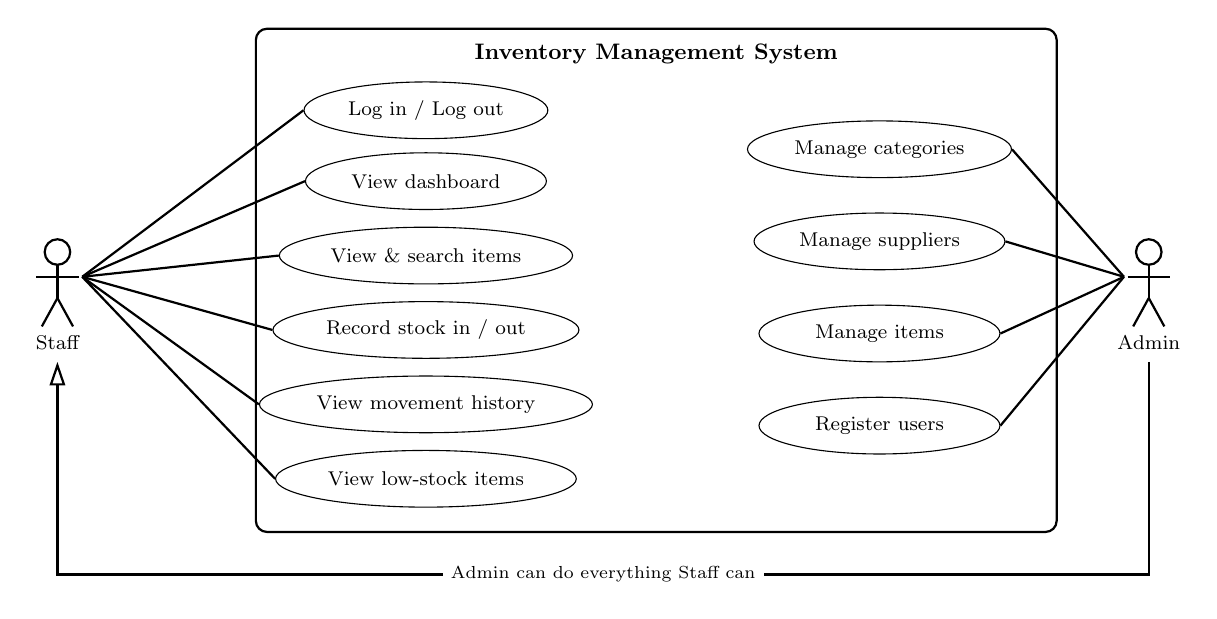
\begin{tikzpicture}[scale=0.9, every node/.style={transform shape}]
  \draw[thick, rounded corners] (-2.4,-6.0) rectangle (8.9,1.1);
  \node[font=\small\bfseries] at (3.25,0.75) {Inventory Management System};
  \node[usecase] (uc1) at (0,-0.05)    {Log in / Log out};
  \node[usecase] (uc2) at (0,-1.05) {View dashboard};
  \node[usecase] (uc3) at (0,-2.1)  {View \& search items};
  \node[usecase] (uc4) at (0,-3.15) {Record stock in / out};
  \node[usecase] (uc5) at (0,-4.2)  {View movement history};
  \node[usecase] (uc6) at (0,-5.25) {View low-stock items};
  \node[usecase] (uc7) at (6.4,-0.6) {Manage categories};
  \node[usecase] (uc8) at (6.4,-1.9) {Manage suppliers};
  \node[usecase] (uc9) at (6.4,-3.2) {Manage items};
  \node[usecase] (uc10) at (6.4,-4.5) {Register users};
  \coordinate (staff) at (-5.2,-2.6);
  \coordinate (admin) at (10.2,-2.6);
  \actor{staff}{Staff}
  \actor{admin}{Admin}
  \foreach \u in {uc1,uc2,uc3,uc4,uc5,uc6} \draw[assoc] (-4.85,-2.4) -- (\u.west);
  \foreach \u in {uc7,uc8,uc9,uc10} \draw[assoc] (9.85,-2.4) -- (\u.east);
  % generalisation: Admin is a Staff (inherits all staff use cases)
  \draw[-{Triangle[open,length=3mm]}, thick] (10.2,-3.6) -- (10.2,-6.6) -- (-5.2,-6.6) -- (-5.2,-3.6);
  \node[font=\scriptsize, fill=white] at (2.5,-6.6) {Admin can do everything Staff can};
\end{tikzpicture}
\caption{Use case diagram}
\label{fig:usecase}
\end{figure}

\subsection{Class Diagram}
\begin{figure}[H]
\centering
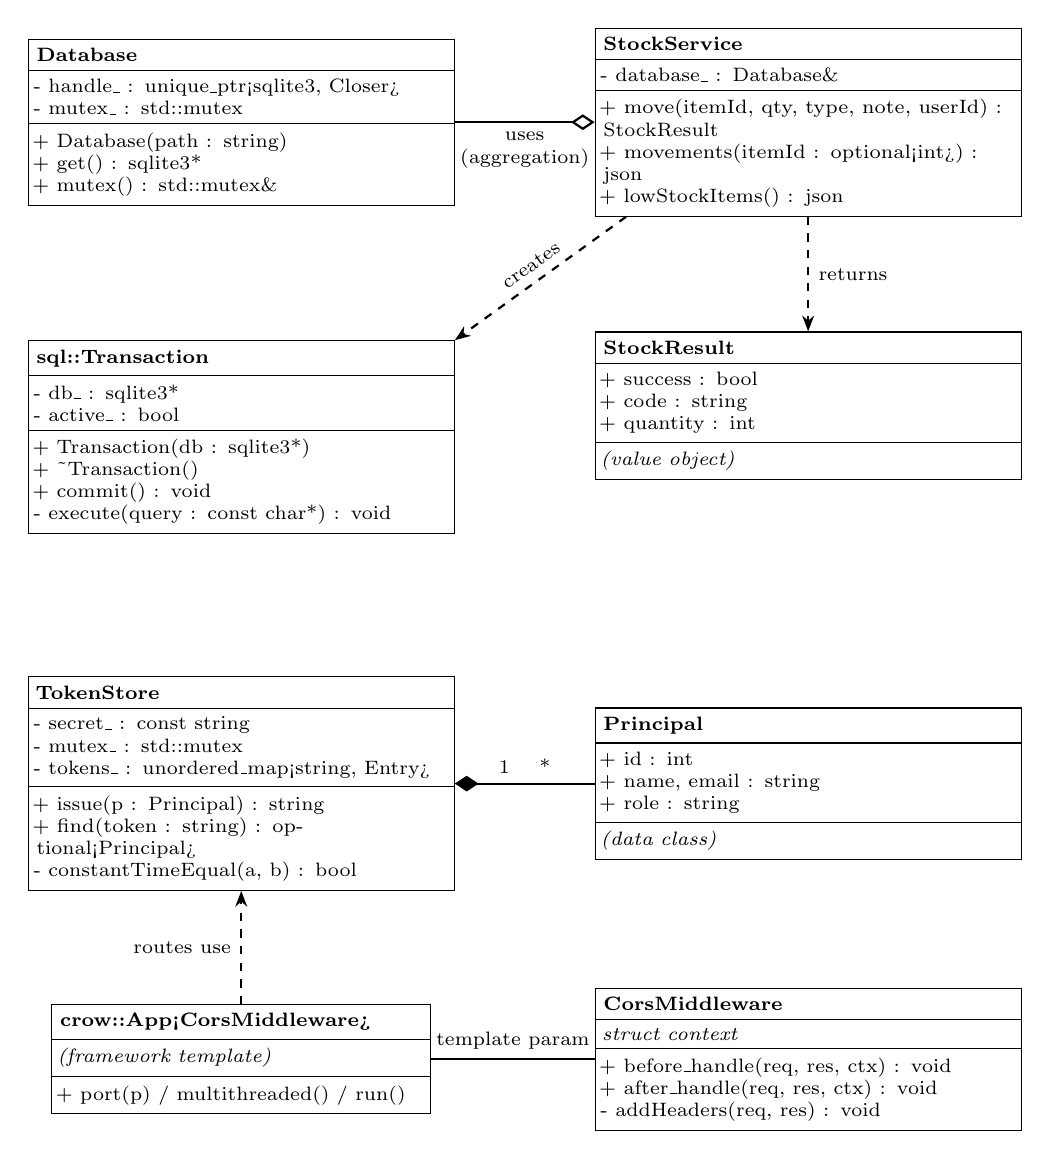
\begin{tikzpicture}[node distance=1.0cm and 0.8cm]
  \node[umlclass] (db) at (0,0) {
    \textbf{\centering Database}
    \nodepart{second}
    - handle\_ : unique\_ptr<sqlite3, Closer>\\
    - mutex\_ : std::mutex
    \nodepart{third}
    + Database(path : string)\\
    + get() : sqlite3*\\
    + mutex() : std::mutex\&};
  \node[umlclass] (ss) at (7.2,0) {
    \textbf{StockService}
    \nodepart{second}
    - database\_ : Database\&
    \nodepart{third}
    + move(itemId, qty, type, note, userId) : StockResult\\
    + movements(itemId : optional<int>) : json\\
    + lowStockItems() : json};
  \node[umlclass] (tx) at (0,-4.0) {
    \textbf{sql::Transaction}
    \nodepart{second}
    - db\_ : sqlite3*\\
    - active\_ : bool
    \nodepart{third}
    + Transaction(db : sqlite3*)\\
    + \textasciitilde Transaction()\\
    + commit() : void\\
    - execute(query : const char*) : void};
  \node[umlclass] (sr) at (7.2,-3.6) {
    \textbf{StockResult}
    \nodepart{second}
    + success : bool\\
    + code : string\\
    + quantity : int
    \nodepart{third}
    \textit{(value object)}};
  \node[umlclass] (ts) at (0,-8.4) {
    \textbf{TokenStore}
    \nodepart{second}
    - secret\_ : const string\\
    - mutex\_ : std::mutex\\
    - tokens\_ : unordered\_map<string, Entry>
    \nodepart{third}
    + issue(p : Principal) : string\\
    + find(token : string) : optional<Principal>\\
    - constantTimeEqual(a, b) : bool};
  \node[umlclass] (pr) at (7.2,-8.4) {
    \textbf{Principal}
    \nodepart{second}
    + id : int\\
    + name, email : string\\
    + role : string
    \nodepart{third}
    \textit{(data class)}};
  \node[umlclass] (cm) at (7.2,-11.9) {
    \textbf{CorsMiddleware}
    \nodepart{second}
    \textit{struct context}
    \nodepart{third}
    + before\_handle(req, res, ctx) : void\\
    + after\_handle(req, res, ctx) : void\\
    - addHeaders(req, res) : void};
  \node[umlclass, text width=4.6cm] (app) at (0,-11.9) {
    \textbf{crow::App<CorsMiddleware>}
    \nodepart{second}
    \textit{(framework template)}
    \nodepart{third}
    + port(p) / multithreaded() / run()};

  \draw[aggr] (ss.west) -- node[below, font=\scriptsize, align=center]{uses\\(aggregation)} (db.east);
  \draw[depend] (ss.south) -- node[right, font=\scriptsize]{returns} (sr.north);
  \draw[depend] ($(ss.south west)+(0.4,0)$) -- node[above, sloped, font=\scriptsize]{creates} (tx.north east);
  \draw[compo] (ts.east) -- node[above, font=\scriptsize]{1 \quad *} (pr.west);
  \draw[assoc] (app.east) -- node[above, font=\scriptsize]{template param} (cm.west);
  \draw[depend] (app.north) -- node[left, font=\scriptsize]{routes use} (ts.south);
\end{tikzpicture}
\caption{Class diagram of the main backend classes}
\label{fig:class}
\end{figure}

\subsection{Sequence Diagram: Stock Out}
\begin{figure}[H]
\centering
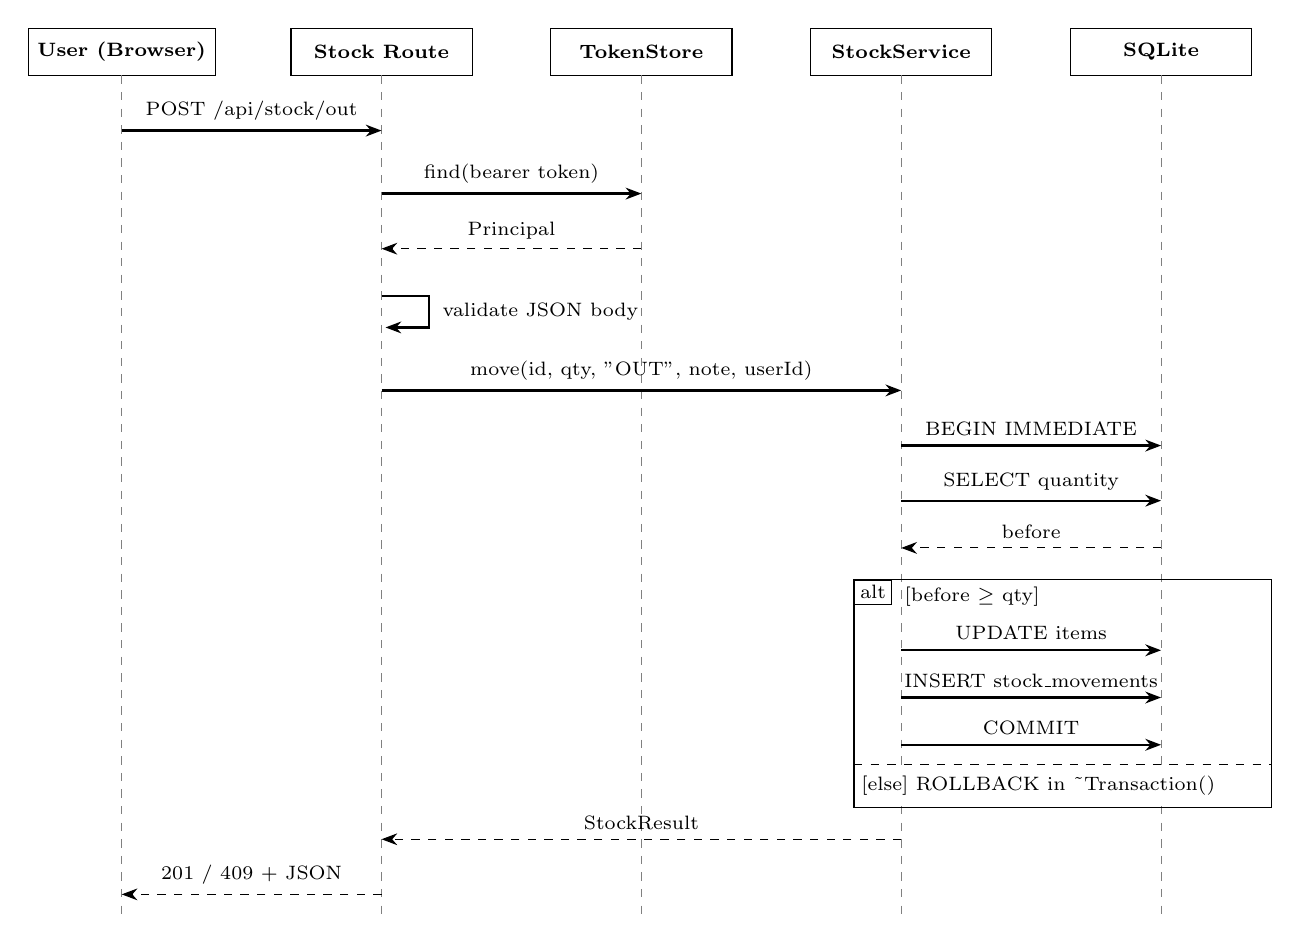
\begin{tikzpicture}[font=\scriptsize]
  \foreach \x/\n/\t in {0/u/User (Browser), 3.3/r/Stock Route, 6.6/t/TokenStore, 9.9/s/StockService, 13.2/d/SQLite} {
    \node[draw, fill=white, minimum width=2.3cm, minimum height=0.6cm, font=\scriptsize\bfseries] (\n) at (\x,0) {\t};
    \draw[dashed, gray] (\x,-0.3) -- (\x,-11.0);
  }
  \draw[msg] (0,-1.0) -- node[above]{POST /api/stock/out} (3.3,-1.0);
  \draw[msg] (3.3,-1.8) -- node[above]{find(bearer token)} (6.6,-1.8);
  \draw[ret] (6.6,-2.5) -- node[above]{Principal} (3.3,-2.5);
  \draw[msg] (3.3,-3.1) -- ++(0.6,0) -- ++(0,-0.4) -- node[above, pos=0.3]{} (3.35,-3.5);
  \node[anchor=west] at (3.95,-3.3) {validate JSON body};
  \draw[msg] (3.3,-4.3) -- node[above]{move(id, qty, "OUT", note, userId)} (9.9,-4.3);
  \draw[msg] (9.9,-5.0) -- node[above]{BEGIN IMMEDIATE} (13.2,-5.0);
  \draw[msg] (9.9,-5.7) -- node[above]{SELECT quantity} (13.2,-5.7);
  \draw[ret] (13.2,-6.3) -- node[above]{before} (9.9,-6.3);
  \draw (9.3,-6.7) rectangle (14.6,-9.6);
  \node[anchor=north west, draw, fill=white, inner sep=2pt] at (9.3,-6.7) {alt};
  \node[anchor=north west, fill=white, inner sep=1pt] at (9.9,-6.75) {[before $\ge$ qty]};
  \draw[msg] (9.9,-7.6) -- node[above]{UPDATE items} (13.2,-7.6);
  \draw[msg] (9.9,-8.2) -- node[above]{INSERT stock\_movements} (13.2,-8.2);
  \draw[msg] (9.9,-8.8) -- node[above]{COMMIT} (13.2,-8.8);
  \draw[dashed] (9.3,-9.05) -- (14.6,-9.05);
  \node[anchor=west, fill=white, inner sep=1pt] at (9.35,-9.32) {[else] ROLLBACK in \textasciitilde Transaction()};
  \draw[ret] (9.9,-10.0) -- node[above]{StockResult} (3.3,-10.0);
  \draw[ret] (3.3,-10.7) -- node[above]{201 / 409 + JSON} (0,-10.7);
\end{tikzpicture}
\caption{Sequence diagram for recording a stock-out}
\label{fig:sequence}
\end{figure}

\subsection{Activity Diagram: Recording a Stock Movement}
\begin{figure}[H]
\centering
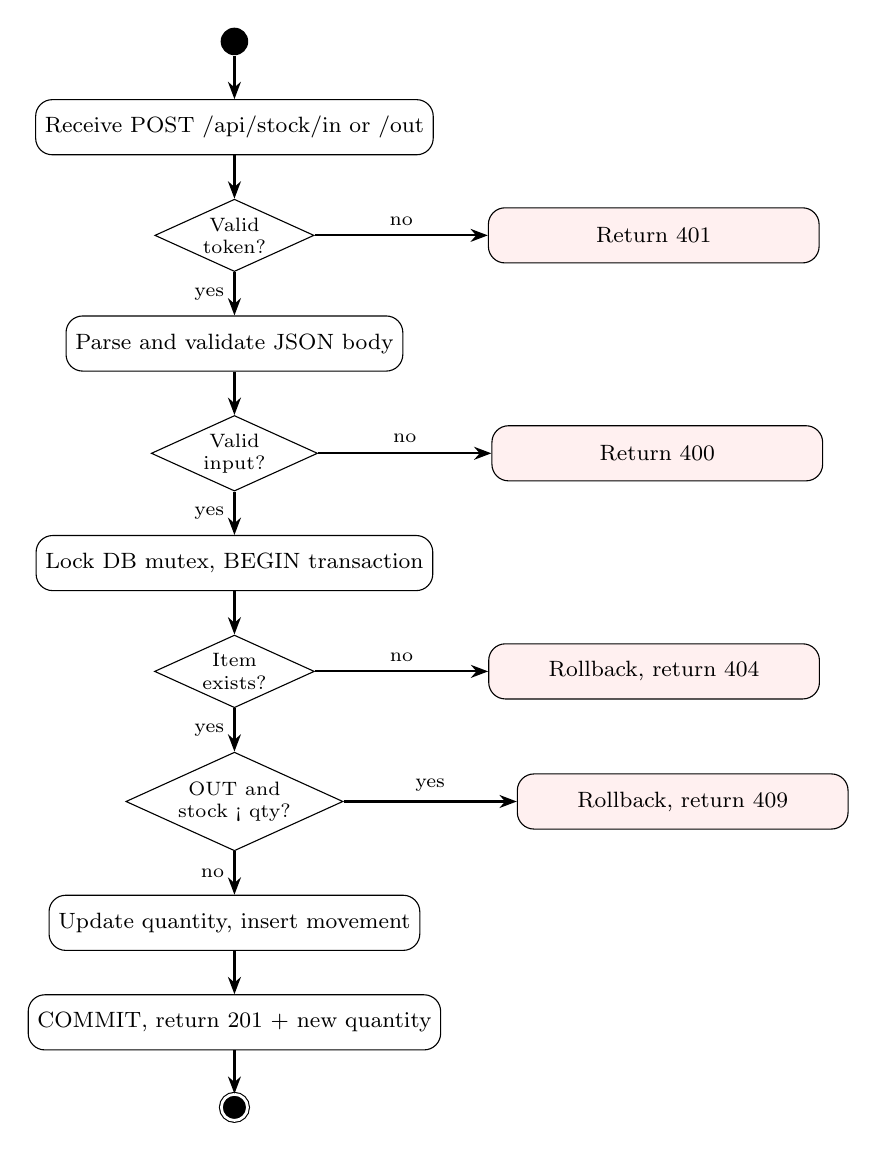
\begin{tikzpicture}[node distance=0.55cm]
  \node[circle, fill=black, minimum size=0.35cm] (start) {};
  \node[act, below=of start] (a1) {Receive POST /api/stock/in or /out};
  \node[dec, below=of a1] (d1) {Valid\\token?};
  \node[act, below=of d1] (a2) {Parse and validate JSON body};
  \node[dec, below=of a2] (d2) {Valid\\input?};
  \node[act, below=of d2] (a3) {Lock DB mutex, BEGIN transaction};
  \node[dec, below=of a3] (d3) {Item\\exists?};
  \node[dec, below=of d3] (d4) {OUT and\\stock < qty?};
  \node[act, below=of d4] (a4) {Update quantity, insert movement};
  \node[act, below=of a4] (a5) {COMMIT, return 201 + new quantity};
  \node[circle, draw, double, double distance=1pt, fill=black, minimum size=0.3cm, below=of a5] (end) {};
  \node[act, right=2.2cm of d1, fill=red!6] (e1) {Return 401};
  \node[act, right=2.2cm of d2, fill=red!6] (e2) {Return 400};
  \node[act, right=2.2cm of d3, fill=red!6] (e3) {Rollback, return 404};
  \node[act, right=2.2cm of d4, fill=red!6] (e4) {Rollback, return 409};
  \draw[flow] (start) -- (a1);
  \draw[flow] (a1) -- (d1);
  \draw[flow] (d1) -- node[left, font=\scriptsize]{yes} (a2);
  \draw[flow] (a2) -- (d2);
  \draw[flow] (d2) -- node[left, font=\scriptsize]{yes} (a3);
  \draw[flow] (a3) -- (d3);
  \draw[flow] (d3) -- node[left, font=\scriptsize]{yes} (d4);
  \draw[flow] (d4) -- node[left, font=\scriptsize]{no} (a4);
  \draw[flow] (a4) -- (a5);
  \draw[flow] (a5) -- (end);
  \draw[flow] (d1) -- node[above, font=\scriptsize]{no} (e1);
  \draw[flow] (d2) -- node[above, font=\scriptsize]{no} (e2);
  \draw[flow] (d3) -- node[above, font=\scriptsize]{no} (e3);
  \draw[flow] (d4) -- node[above, font=\scriptsize]{yes} (e4);
\end{tikzpicture}
\caption{Activity diagram for the stock in/out workflow}
\label{fig:activity}
\end{figure}

\section{Implementation: Key Code Snippets}

\subsection{RAII Database Wrapper (Encapsulation and Composition)}
\begin{lstlisting}[caption={\texttt{Database} class: owns the SQLite connection and its mutex}, label={lst:db}]
class Database {
  public:
    explicit Database(const std::string &path);
    sqlite3 *get() const noexcept { return handle_.get(); }
    std::mutex &mutex() noexcept { return mutex_; }

  private:
    struct Closer {
        void operator()(sqlite3 *db) const noexcept { if (db) sqlite3_close(db); }
    };
    std::unique_ptr<sqlite3, Closer> handle_;   // closed automatically
    std::mutex mutex_;
};
\end{lstlisting}

\subsection{Transaction Class (RAII and Copy Control)}
\begin{lstlisting}[caption={\texttt{sql::Transaction}: rollback in the destructor unless committed}, label={lst:tx}]
class Transaction {
  public:
    explicit Transaction(sqlite3 *db) : db_(db) { execute("BEGIN IMMEDIATE"); }
    Transaction(const Transaction &) = delete;              // non-copyable
    Transaction &operator=(const Transaction &) = delete;
    ~Transaction() {
        if (active_) sqlite3_exec(db_, "ROLLBACK", nullptr, nullptr, nullptr);
    }
    void commit() { execute("COMMIT"); active_ = false; }

  private:
    void execute(const char *query);   // throws std::runtime_error on failure
    sqlite3 *db_;
    bool active_ = true;
};
\end{lstlisting}

\subsection{Business Logic in the Service Layer (Abstraction)}
\begin{lstlisting}[caption={\texttt{StockService::move()} (abridged): atomic stock update and movement log}, label={lst:move}]
StockResult StockService::move(int itemId, int amount, const std::string &type,
                               const std::string &note, int userId) {
    if (itemId <= 0 || amount <= 0 || userId <= 0 || (type != "IN" && type != "OUT"))
        return {false, "INVALID_INPUT", 0};
    try {
        std::lock_guard<std::mutex> lock(database_.mutex());
        sql::Transaction transaction(database_.get());
        auto lookup = sql::prepare(database_.get(),
                                   "SELECT quantity FROM items WHERE id=?");
        sql::bindInt(lookup.get(), 1, itemId);
        if (sqlite3_step(lookup.get()) != SQLITE_ROW) return {false, "ITEM_NOT_FOUND", 0};
        const int before = sqlite3_column_int(lookup.get(), 0);
        if (type == "OUT" && before < amount) return {false, "INSUFFICIENT_STOCK", before};
        // ... UPDATE items ..., then INSERT INTO stock_movements(...) ...
        transaction.commit();                       // otherwise destructor rolls back
        return {true, "", type == "IN" ? before + amount : before - amount};
    } catch (const std::exception &) {
        return {false, "DATABASE_ERROR", 0};
    }
}
\end{lstlisting}

\subsection{Token Store (Encapsulation)}
\begin{lstlisting}[caption={\texttt{TokenStore}: private state behind a two-method interface (abridged)}, label={lst:token}]
struct Principal { int id{}; std::string name; std::string email; std::string role; };

class TokenStore {
  public:
    std::string issue(Principal principal);                  // nonce + "." + HMAC
    std::optional<Principal> find(const std::string &token); // verify + expiry check
  private:
    static bool constantTimeEqual(const std::string &l, const std::string &r);
    struct Entry { Principal principal; std::chrono::system_clock::time_point expires; };
    const std::string secret_ = password::randomSalt();
    std::mutex mutex_;
    std::unordered_map<std::string, Entry> tokens_;
};
\end{lstlisting}

\subsection{Polymorphism: Function Overloading and Template Middleware}
\begin{lstlisting}[caption={Overloaded \texttt{response::success()} and the middleware passed as a template argument}, label={lst:poly}]
namespace inventory::response {
inline crow::response success(const nlohmann::json &data, int status = 200);
inline crow::response success(crow::json::wvalue data, int status = 200);
inline crow::response error(int status, const std::string &message);
}

struct CorsMiddleware {
    struct context {};
    void before_handle(crow::request &req, crow::response &res, context &);
    void after_handle(crow::request &req, crow::response &res, context &);
};

crow::App<CorsMiddleware> app;   // static polymorphism via templates
inventory::routes::registerStockRoutes(app, stockService, tokens);
app.port(8080).multithreaded().run();
\end{lstlisting}

\section{Project Screenshots}
The screenshots below were taken from the Stockroom frontend running against the C++ backend
at \texttt{http://localhost:8080}. The ``API connected'' indicator in the sidebar confirms
that the browser is talking to the REST API.

\begin{figure}[H]
\centering
\fbox{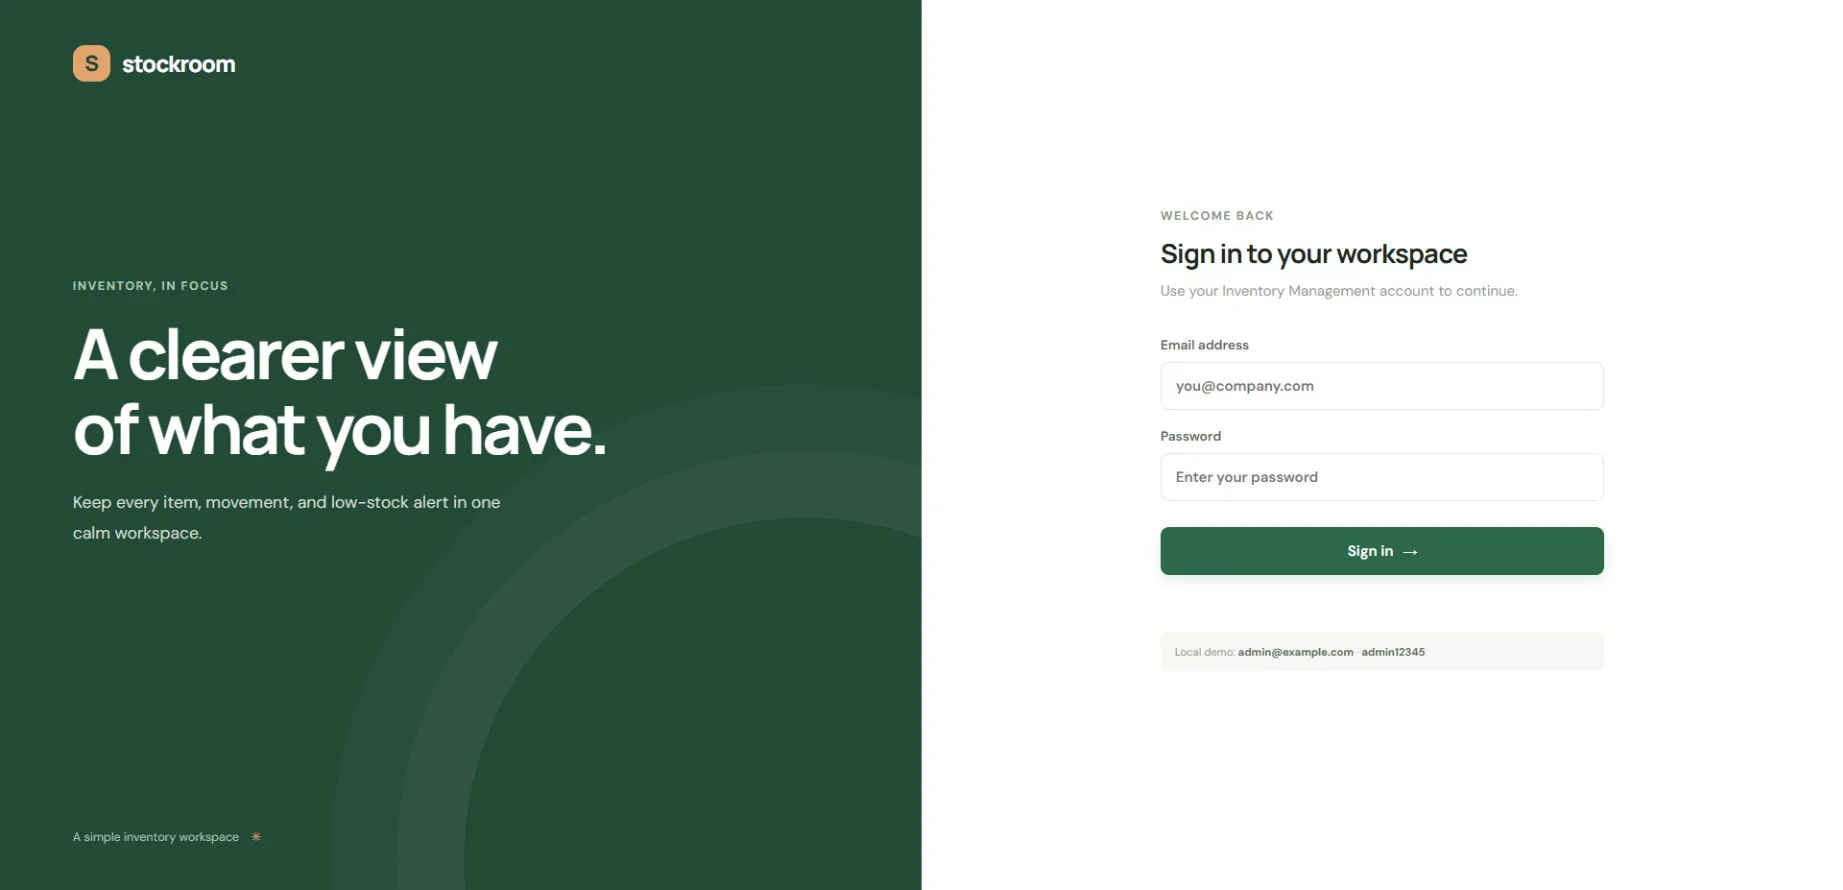
\includegraphics[width=0.86\linewidth]{shots/ss1.png}}
\caption{Sign-in page: credentials are sent to \texttt{POST /api/auth/login}, which returns a bearer token}
\label{fig:ss-login}
\end{figure}

\begin{figure}[H]
\centering
\fbox{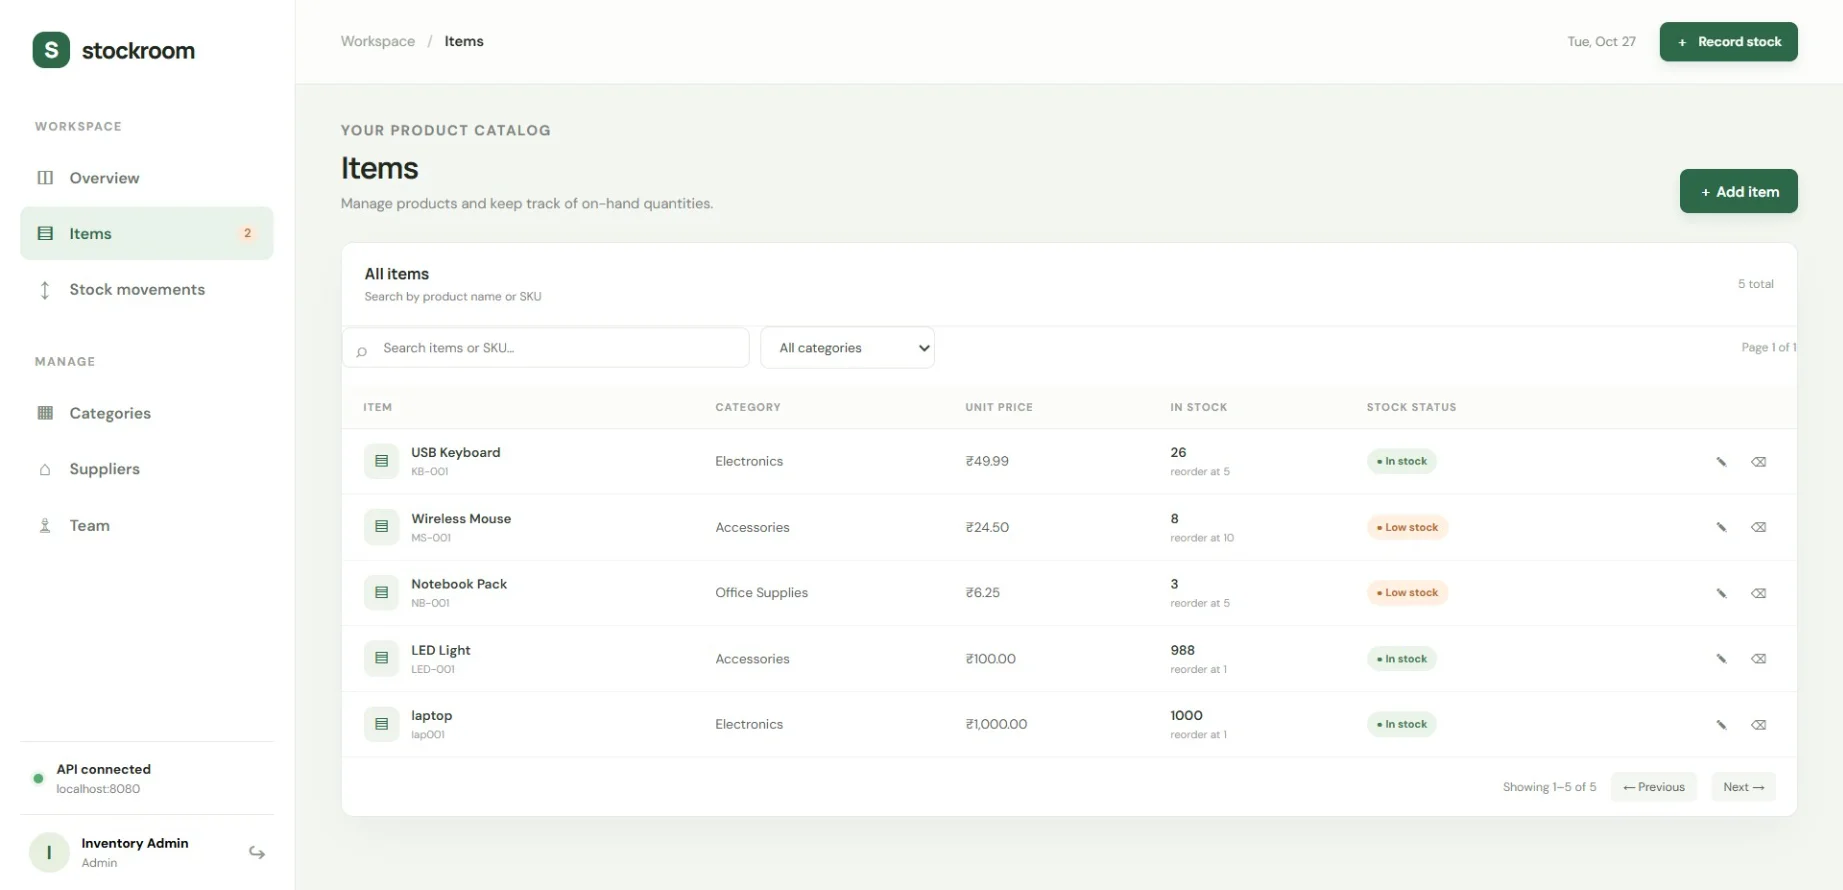
\includegraphics[width=0.86\linewidth]{shots/ss4.png}}
\caption{Items catalogue with search, category filter, pagination and low-stock status (\texttt{GET /api/items})}
\label{fig:ss-items}
\end{figure}

\begin{figure}[H]
\centering
\fbox{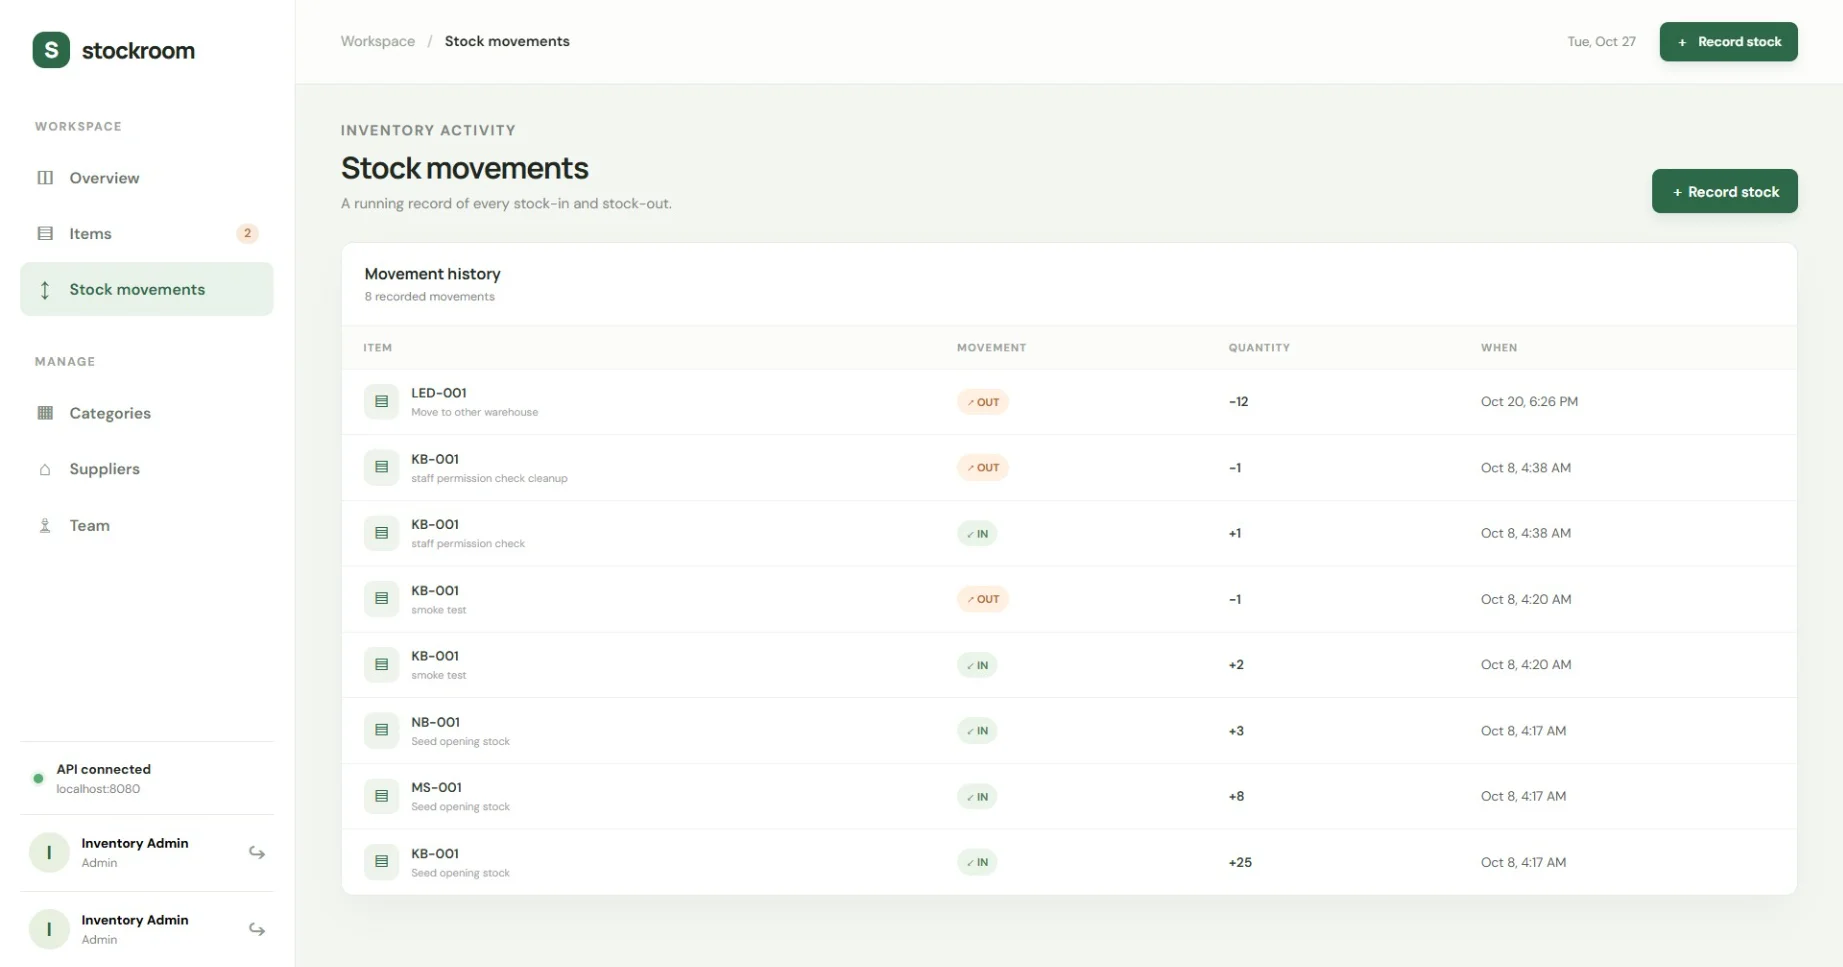
\includegraphics[width=0.86\linewidth]{shots/ss2.png}}
\caption{Stock movement history recorded by \texttt{StockService} (\texttt{GET /api/stock/movements})}
\label{fig:ss-movements}
\end{figure}

\begin{figure}[H]
\centering
\fbox{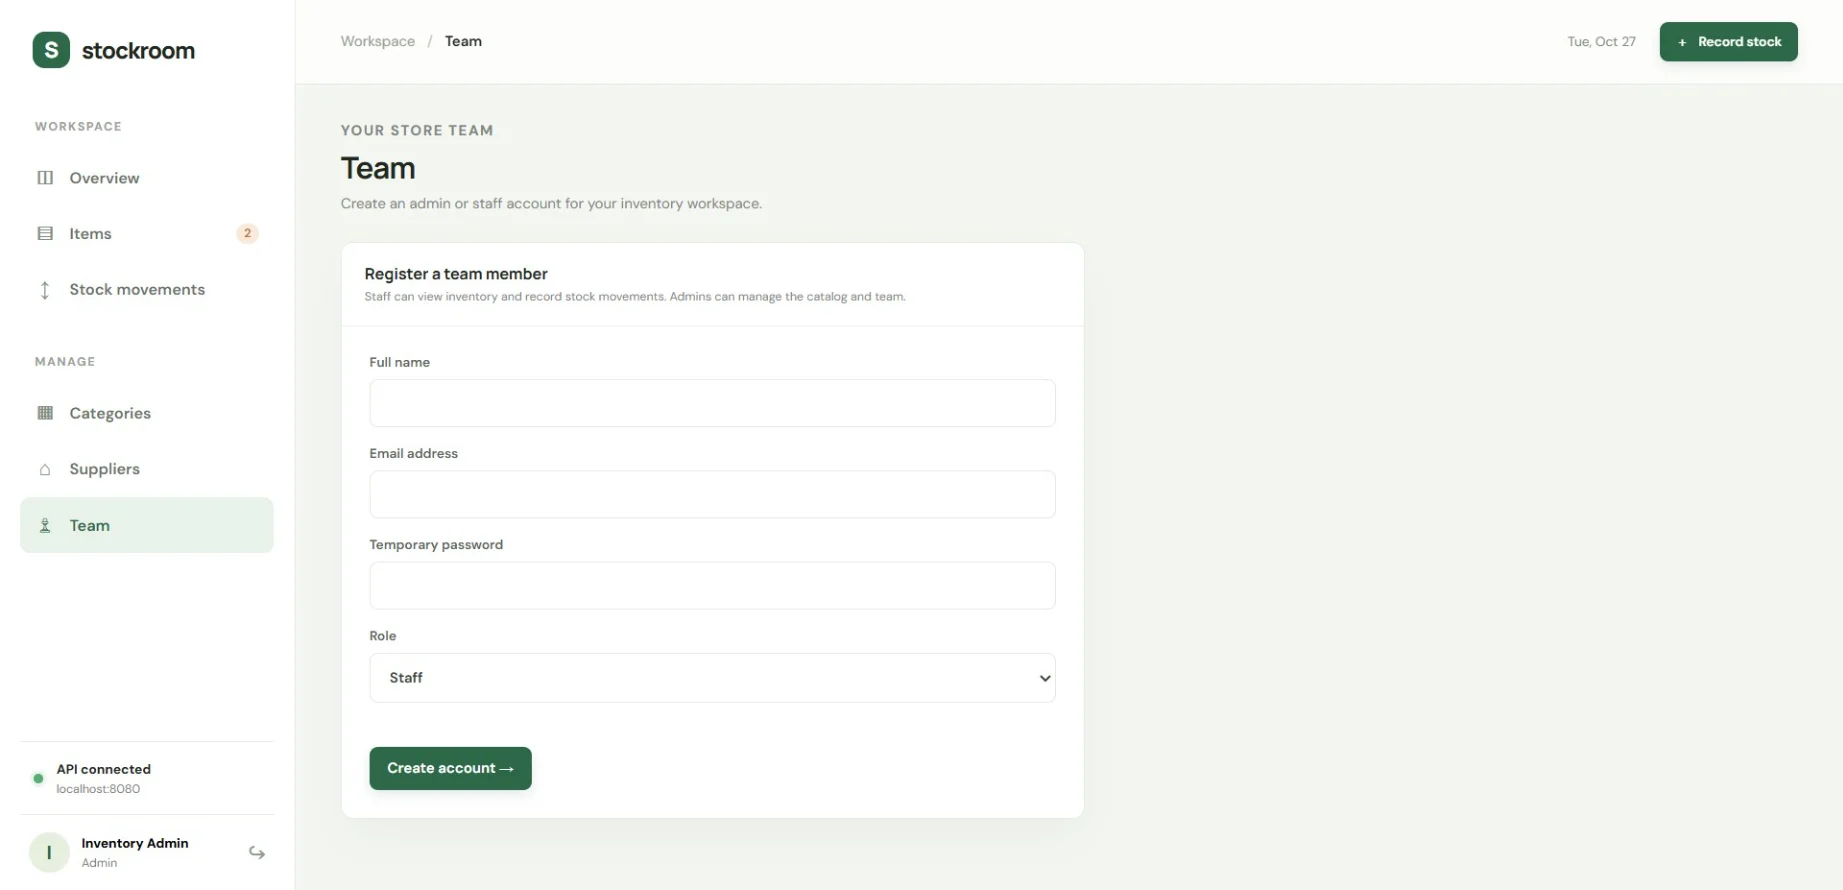
\includegraphics[width=0.86\linewidth]{shots/ss3.png}}
\caption{Team page: an admin registers a staff or admin account (\texttt{POST /api/auth/register})}
\label{fig:ss-team}
\end{figure}

\section{Conclusion and Future Work}
The Inventory Management System integrates a browser frontend, a C++17 REST API and an
SQLite database into one end-to-end workflow. Classes such as \texttt{Database},
\texttt{sql::Transaction}, \texttt{StockService} and \texttt{TokenStore} show encapsulation,
abstraction, RAII, composition, aggregation and polymorphism in practice. Transactional stock
updates keep quantities and the movement history consistent.

Future work includes reading secrets (such as the token signing key) from environment
variables with \texttt{std::getenv}, using stronger password hashing (bcrypt or Argon2),
persistent sessions, support for multiple warehouses, purchase and sales orders, CSV/PDF
reports, and automated tests.

\end{document}
